\documentclass[11pt,a4paper]{book}
\usepackage[a4paper,
            left=1.75 cm,
            right=1.75 cm,
            top=2.95 cm,
            bottom=3.2 cm,
]{geometry}

\usepackage[dvipsnames]{xcolor}

\setlength{\parindent}{0pt}

\definecolor{myblue}{rgb}{0, 0, 0.65}

\newcounter{question}

\setcounter{question}{0}

\newcommand\Que[1]{
    \rule{\textwidth}{0.02cm}
    \stepcounter{question}
    \fbox{{\color{red}\thequestion. Q}}  {\color{myblue}   #1}\par}

\newcommand\Ans[1]{
    \fbox{{\color{blue} \thequestion. A}}  {  #1}\par}


\usepackage{tikz}
\usetikzlibrary{matrix}
\tikzset{ 
    table/.style={
        matrix of nodes,
        row sep=-\pgflinewidth,
        column sep=-\pgflinewidth,
        nodes={rectangle,minimum width=3em,align=center},
        text depth=1.25ex,
        text height=2.5ex,
        nodes in empty cells
    },
row 1/.style={nodes={fill=green!10,text depth=0.4ex,text height=2ex}},
row 6/.style={nodes={text depth=0.4ex,text height=2ex}},
column 1/.style={nodes={fill=green!10}, minimum width=7em,text width=3.5cm},
}





\begin{document}

\begin{large}
  {\bf \boldmath

    \Que{
      The binary sequence \texttt{10010110010} is the input to the precoder whose output is used to modulate a duobinary transmitting filter. Construct a table  showing the precoded sequence, the transmitted amplitude levels, the received signal levels, and the decoded sequence.
    }


    \Ans{}

    \begin{footnotesize}
      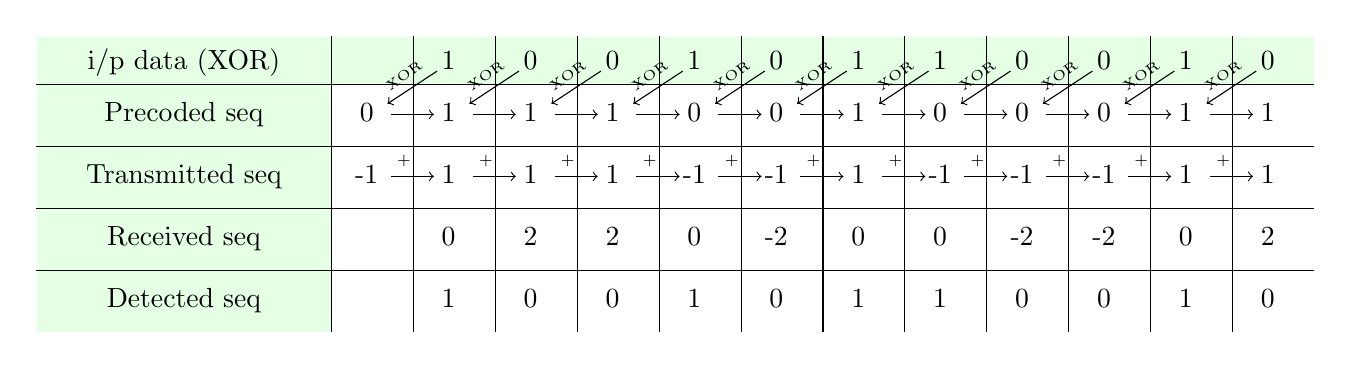
\begin{tikzpicture}
        % the matrix entries
        \matrix (mat) [table]
        {
          i/p data (XOR)  &    & 1 & 0 & 0 & 1  & 0  & 1 & 1  & 0  & 0  & 1 & 0 \\
          Precoded seq    & 0  & 1 & 1 & 1 & 0  & 0  & 1 & 0  & 0  & 0  & 1 & 1 \\
          Transmitted seq & -1 & 1 & 1 & 1 & -1 & -1 & 1 & -1 & -1 & -1 & 1 & 1 \\
          Received seq    &    & 0 & 2 & 2 & 0  & -2 & 0 & 0  & -2 & -2 & 0 & 2 \\
          Detected seq    &    & 1 & 0 & 0 & 1  & 0  & 1 & 1  & 0  & 0  & 1 & 0 \\
        };
        the matrix rules
        \foreach \x in {1,...,4}
          {
            \draw
            ([xshift=-.5\pgflinewidth]mat-\x-1.south west) --
            ([xshift=-.5\pgflinewidth]mat-\x-13.south east);
          }
        \foreach \x in {1,...,12}
          {
            \draw
            ([yshift=.5\pgflinewidth]mat-1-\x.north east) --
            ([yshift=.5\pgflinewidth]mat-5-\x.south east);
          }
        % the arrows
        \begin{scope}[shorten >=7pt,shorten <= 7pt]
          % \foreach \x in {2,...,5}
          % {
          \draw[->]  (mat-1-3.center) -- node[above, font=\tiny,rotate=35] { XOR}  (mat-2-2.center);
          \draw[->]  (mat-2-2.center) --    (mat-2-3.center);
          \draw[->]  (mat-1-4.center) -- node[above, font=\tiny,rotate=35] { XOR}  (mat-2-3.center);
          \draw[->]  (mat-2-3.center) --    (mat-2-4.center);
          \draw[->]  (mat-1-5.center) -- node[above, font=\tiny,rotate=35] { XOR}  (mat-2-4.center);
          \draw[->]  (mat-2-4.center) --    (mat-2-5.center);
          \draw[->]  (mat-1-6.center) -- node[above, font=\tiny,rotate=35] { XOR}  (mat-2-5.center);
          \draw[->]  (mat-2-5.center) --    (mat-2-6.center);
          \draw[->]  (mat-1-7.center) -- node[above, font=\tiny,rotate=35] { XOR}  (mat-2-6.center);
          \draw[->]  (mat-2-6.center) --    (mat-2-7.center);
          \draw[->]  (mat-1-8.center) -- node[above, font=\tiny,rotate=35] { XOR}  (mat-2-7.center);
          \draw[->]  (mat-2-7.center) --    (mat-2-8.center);
          \draw[->]  (mat-1-9.center) -- node[above, font=\tiny,rotate=35] { XOR}  (mat-2-8.center);
          \draw[->]  (mat-2-8.center) --    (mat-2-9.center);
          \draw[->]  (mat-1-10.center) -- node[above, font=\tiny,rotate=35] { XOR}  (mat-2-9.center);
          \draw[->]  (mat-2-9.center) --    (mat-2-10.center);
          \draw[->]  (mat-1-11.center) -- node[above, font=\tiny,rotate=35] { XOR}  (mat-2-10.center);
          \draw[->]  (mat-2-10.center) --    (mat-2-11.center);
          \draw[->]  (mat-1-12.center) -- node[above, font=\tiny,rotate=35] { XOR}  (mat-2-11.center);
          \draw[->]  (mat-2-11.center) --    (mat-2-12.center);
          \draw[->]  (mat-1-13.center) -- node[above, font=\tiny,rotate=35] { XOR}  (mat-2-12.center);
          \draw[->]  (mat-2-12.center) --    (mat-2-13.center);

          \draw[->]  (mat-3-2.center) --   node[above, font=\tiny, xshift=-3px] {+}  (mat-3-3.center);
          \draw[->]  (mat-3-3.center) --   node[above, font=\tiny, xshift=-3px] {+}  (mat-3-4.center);
          \draw[->]  (mat-3-4.center) --   node[above, font=\tiny, xshift=-3px] {+}  (mat-3-5.center);
          \draw[->]  (mat-3-5.center) --   node[above, font=\tiny, xshift=-3px] {+}  (mat-3-6.center);
          \draw[->]  (mat-3-6.center) --   node[above, font=\tiny, xshift=-3px] {+}  (mat-3-7.center);
          \draw[->]  (mat-3-7.center) --   node[above, font=\tiny, xshift=-3px] {+}  (mat-3-8.center);
          \draw[->]  (mat-3-8.center) --   node[above, font=\tiny, xshift=-3px] {+}  (mat-3-9.center);
          \draw[->]  (mat-3-9.center) --   node[above, font=\tiny, xshift=-3px] {+}  (mat-3-10.center);
          \draw[->]  (mat-3-10.center) --  node[above, font=\tiny, xshift=-3px] {+}   (mat-3-11.center);
          \draw[->]  (mat-3-11.center) --  node[above, font=\tiny, xshift=-3px] {+}   (mat-3-12.center);
          \draw[->]  (mat-3-12.center) --  node[above, font=\tiny, xshift=-3px] {+}   (mat-3-13.center);
        \end{scope}
      \end{tikzpicture}
    \end{footnotesize}

  }

\end{large}
\end{document}
